\documentclass[11pt, A4paper,norsk]{article}
\usepackage[utf8]{inputenc}
\usepackage[T1]{fontenc}
\usepackage{babel}
\usepackage{amsmath}
\usepackage{amsfonts}
\usepackage{amsthm}
\usepackage{amssymb}
\usepackage[colorlinks]{hyperref}
\usepackage{listings}
\usepackage{color}
\usepackage{hyperref}
\usepackage{graphicx}
\usepackage{cite}
\usepackage{textcomp}
\usepackage{float}

\definecolor{dkgreen}{rgb}{0,0.6,0}
\definecolor{gray}{rgb}{0.5,0.5,0.5}
\definecolor{daynineyellow}{rgb}{1.0,0.655,0.102}
\definecolor{url}{rgb}{0.1,0.1,0.4}

\lstset{frame=tb,
	language=Python,
	aboveskip=3mm,
	belowskip=3mm,
	showstringspaces=false,
	columns=flexible,
	basicstyle={\small\ttfamily},
	numbers=none,
	numberstyle=\tiny\color{gray},
	keywordstyle=\color{blue},
	commentstyle=\color{daynineyellow},
	stringstyle=\color{dkgreen},
	breaklines=true,
	breakatwhitespace=true,
	tabsize=3
}

\lstset{inputpath="C:/Users/Torstein/Documents/UiO/Fys2130/Python programmer"}
\graphicspath{{C:/Users/Torstein/Documents/UiO/Fys2130/"Python programmer"/}}
\hypersetup{colorlinks, urlcolor=url}

\author{Torstein Solheim Ølberg}
\title{Svar på Oblig nr. 7 i Fys2130}



%\lstinputlisting{Filnavn! type kodefil}
%\includegraphics[width=12.6cm,height=8cm]{Filnavn! type png}



\begin{document}
\maketitle
	\begin{center}
\Large \textbf{Oppgaver}
	\end{center}









		\paragraph{8.}
			\begin{flushleft}
Hvis du plasserer en gjendstand forran linsa og en skjerm på den andre siden av linsa er brenvidden gitt av
$$f = \frac{1}{\frac{1}{s} + \frac{1}{s'}} = \frac{s s'}{s' + s}$$
der $s'$ er avstanden fra linsa til der skjermen har et skarpt bilde av gjenstanden vi plasserte, og $s$ er avstanden fra gjenstanden til linsa. Dette er en veldig omtrentlig utregning med mindre du bruker veldig nøyaktig måling, men da går det ikke så raskt.
			\end{flushleft}









		\paragraph{11.}
			\begin{flushleft}
Grunnen til at du ser uskarpt når du ser under vann, er fordi vann og luft har forskjellige brytningskonstanter. Siden øyet ditt er vant til å se lys som kommer fra luft, vil ikke lyset fokuseres i riktig punkt på netthinna. Derfor blir bildet uskarpt. \\

Med de riktige brillene kunne du klart deg uten noe luft noe sted, men da er brillene nødt til å være konveks, siden brytningsindeksen til vann er større enn luft, som vil si at lyset fokuseres lengre bak enn netthinna. Det betyr at vi trenger å samle lyset tidligere, som vi kan gjøre med en ekstra samlelinse. Denne må bare være spesiallaget utifra hva slags vann man befinner seg i.
			\end{flushleft}









		\paragraph{15.}
			\begin{flushleft}
Siden innfallsvinkel er lik utfallsvinkel for refleksjon, så er et speil som skal vise hele kroppen din nødt til å være minst like stor som halvparten av kroppsstørrelsen din. Det kommer av at lyset som kommer fra tærne dine da må treffe speilet i høyden halvveis opp til øyet. \\

Speilet må også være plassert slik at toppen av speilet er like høyt som øynene til personen som skal se i dem. \\

Når det gjelder avstanden til speilet så spiller ikke den noen rolle, siden alt vi bryr oss noe om når vi skal se oss selv er at lyset treffer halveis opp på veggen til øynene dine, og siden denne høyden ikke endres med avstanden fra speilet så skjer det ingenting. Står du for langt unna vil du selvfølgelig ikke kunne se deg selv fordi for lite av lyset kommer til øynene dine, men teoretisk sett kan du se hele kroppen, hvis det hadde vært nok lys.
			\end{flushleft}
			












		\paragraph{17.} $ $
			\begin{figure}[H]
\label{13}
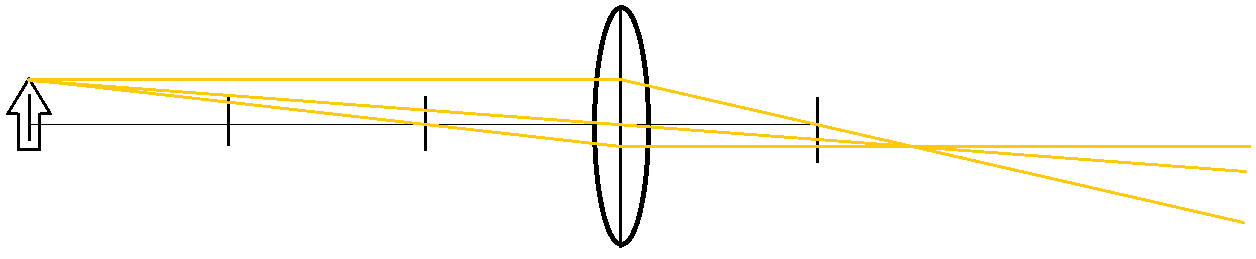
\includegraphics[width=12.6cm, height=7cm]{Figur_0013.png}
\caption{Tegning av lys fra objekt gjennom en linse, med avstand $3$ brennvidder.}
			\end{figure}
			\begin{flushleft}
Vi ser her \ref{13} at når objektet befinner seg $3$ brennvidder unna linsa vil lyset som kommer fra ett punkt blir samlet veldig nærme en brennvidde, men opp ned. Dette blidet vil bli reelt, og litte grann mindre enn det orginale objektet.
			\end{flushleft}
			\begin{figure}[H]
\label{14}
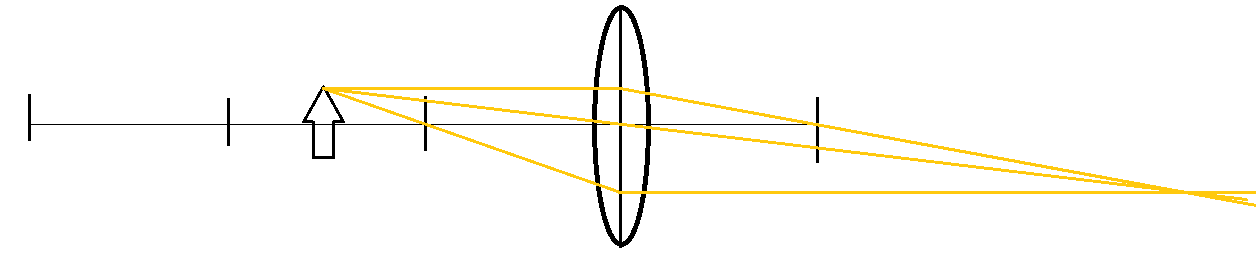
\includegraphics[width=12.6cm, height=7cm]{Figur_0014.png}
\caption{Tegning av lys fra objekt gjennom en linse, med avstand $1.5$ brennvidder.}
			\end{figure}
			\begin{flushleft}
Når vi beveger oss nærmere en brennvidde med objektet vårt vil samlingspunktet bli lavere og lengere fra linsa, slik som vi ser i dette \ref{14} bildet. Blirdet vil derfor fortsatt være reelt, men denne gangen er blidet mye større en det faktiske objektet
			\end{flushleft}
			\begin{figure}[H]
\label{15}
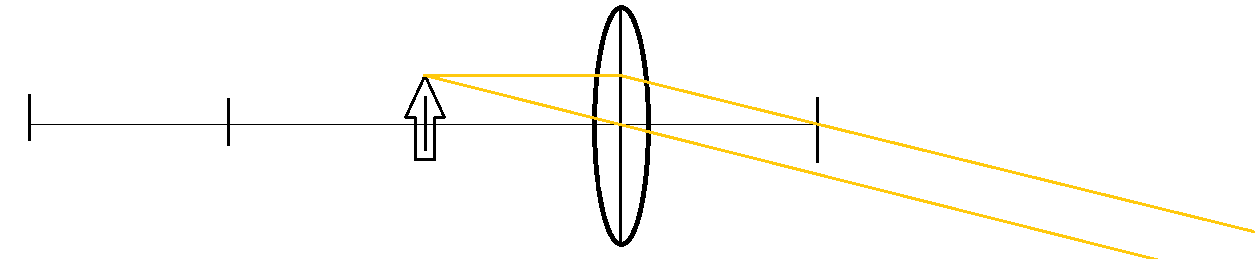
\includegraphics[width=12.6cm, height=7cm]{Figur_0015.png}
\caption{Tegning av lys fra objekt gjennom en linse, med avstand $1$ brennvidde.}
			\end{figure}
			\begin{flushleft}
I dette blidet \ref{15} kan vi se at når objektet passerer en brenvidde i posisjon vil lysstrålene ikke lenger samles, men være parallele. I tillegg vil det ikke være noen vits i å tegne inn lysstrålen som passerer gjennom den første brennvidden, fordi denne lysstrålen vil gå loddrett opp, og derfor aldri ha muligheten til å passere gjennom linsa. Eneste unntaket er hvis lyset kommer fra et punkt som er både på objektet og fra der brenviddestreken krysser den optiske aksen. Da er alle tre strekene oppå hverandre og vil alltid være samlet.
			\end{flushleft}
			\begin{figure}[H]
\label{16}
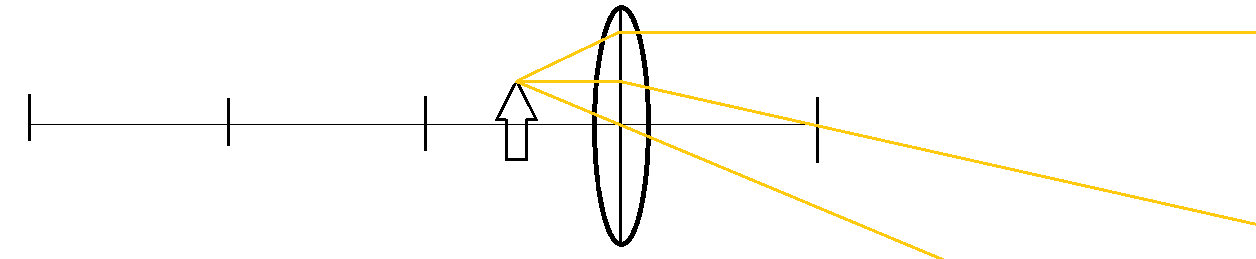
\includegraphics[width=12.6cm, height=7cm]{Figur_0016.png}
\caption{Tegning av lys fra objekt gjennom en linse, med avstand $0.5$ brennvidder.}
			\end{figure}
			\begin{flushleft}
Tilslutt ser vi et bilde \ref{16} med objektet flyttet nærmere enn en brennvidde. Nå vil ikke lenger lensa virke samlende, men heller spredende på høyre side. På venstre side er derimot linsa samlende, og det vil dannes et virtuelt bilde. Dette bildet vil være av et mye større objekt en det opprinnelige objektet, og i motsettning til alle tidligere ganger vil dette objektet være riktig vei.
			\end{flushleft}










		\paragraph{23.}
			\begin{flushleft}
Fra linseformelen har vi at hvis brennvidden $f = 85 \text{mm}$ og avstanden til linsa $s = 3.5 \text{m}$ så er avstanden til bildeplanet $s'$ gitt ved
$$s' = \frac{fs}{s - f} = \frac{85 \cdot 10^{-3} \text{m} \cdot 3.5 \text{m}}{3.5 \text{m} - 85 \cdot 10^{-3} \text{m}} = 0.0871 \text{m}$$
Fra uttrykket for lineær forstørrelse har vi at
$$|M| = \frac{s'}{s} = \frac{0.087 \text{m}}{3.5 \text{m}} = 0.0249$$
som vil si at høyden til personen på bildet er gitt av
$$h \cdot |M| = 1.75 \text{m} \cdot 0.0249 = 0.044 \text{m} = 44 \text{mm}$$
som er mer enn den lengste siden av bildedrikken. Det vil si at vi ikke får med hele personen. Dette virker veldig urealtistisk i forholdt til hvor bra mobilkameraet mitt er nå, men det kan allikevel hende dette er riktig, siden bildet blir lagret på en gammeldags film. Vet dessverre ikke nok om størrelsen på bildebrikka til en normal telefon nå. \\

Hvis bildet blir lagret på en brikke med den lengste siden lik $23.6 \text{mm}$ vil $\frac{44 \text{mm} - 23.6 \text{mm}}{44 \text{mm}} = \frac{20.4}{44} = 0.46 = 46 \%$ av personen komme med på bildet, eller ca. halvparten.
			\end{flushleft}









		\paragraph{30.}
			\subparagraph{a)}
				\begin{flushleft}
foreskriver optikkeren en brille med linsestyrke på $2.75 \text{dioptre}$  betyr det at personen sin linsestyrke er på $54 \text{dioptre} - 2.75 \text{dioptre} = 51.25 \text{dioptre}$. Det vil da si at likningen for avstanden til nærpunktet blir
$$x = \frac{1}{\frac{1}{f} - \frac{1}{0.02 \text{m}}} = \frac{1}{51.25 \text{dioptre} - 50 \text{dioptre}} = 0.8 \text{m}$$
Altså er personen sitt nærpunkt ved en avstand på $80 \text{cm}$.
				\end{flushleft}










			\subparagraph{b)}
				\begin{flushleft}
For en person som blir foreskrevet en brille med styrke på $-1.30 \text{dioptre}$ får vi at personen sin linsestyrke er $50 \text{dioptre} + 1.30 \text{dioptre} = 51.30 \text{dioptre}$. Altså vil avstanden til fjernpyunktet for denne persoen bli gitt av
$$x = \frac{1}{\frac{1}{f} - \frac{1}{0.02 \text{m}}} = \frac{1}{51.30 \text{dioptre} - 50 \text{dioptre}} = 0.77 \text{m}$$
Altså at avstanden til fjærnpunktet ligger $77 \text{cm}$ unna.
				\end{flushleft}









		\paragraph{40.}
			\subparagraph{a)}
				\begin{flushleft}
Så lenge objektet er plassert på eller rett utenfor brennpunktet til objektivet, altså $8.0 \text{mm}$ unna objektivet, fungerer mikroskopet, men det er lurt å plassere det så nærme brennpunktet som mulig.
				\end{flushleft}












			\subparagraph{b)}
				\begin{flushleft}
Forstørrelsen fra objektivet aleine er gitt ved
$$M_1 = \frac{s_1'}{s_1} = \frac{197 \text{mm} - 18 \text{mm}}{8.0 \text{mm}} = \frac{179}{8.0} = 22.375$$
der $s_1'$ er avstanden fra objektivet til brennvidden av okularet, og $s_1$ er avstanden fra objektivet til brennvidden til objektivet.
				\end{flushleft}












			\subparagraph{c)}
				\begin{flushleft}
Okularet aleine gir en forstørring gitt av
$$M_2 = \frac{250 \text{mm}}{f_2} = \frac{250 \text{mm}}{18 \text{mm}} = 13.9$$
der $250 \text{mm}$ er brennvidden til øyetlinsa, og $f_2$ er brennvidden til okularet.
				\end{flushleft}









			\subparagraph{d)}
				\begin{flushleft}
Den totale forstørelsen for et mikroskop er definert som $M_{\text{tot}} = M_1 \cdot M_2$ og hvis vi setter inn uttrykkene for disse $M$ene, som vi har fra de to forrige oppgavene, får vi
$$M_{\text{tot}} = \frac{25 \text{cm} s_1'}{f_2 s_1}$$
				\end{flushleft}










			\subparagraph{e)}
				\begin{flushleft}
Dette mikroskopet har en forstørrelse på
$$M_{\text{tot}} = 22.375 \cdot 13.9 = 311 \approx 310 X$$
				\end{flushleft}
\end{document}